\documentclass[11pt]{article}

\usepackage[margin=1in]{geometry}
\usepackage[T1]{fontenc}
\usepackage[utf8]{inputenc}
\usepackage{lmodern}
\usepackage{microtype}
\usepackage{graphicx}
\usepackage{booktabs}
\usepackage{multirow}
\usepackage{array}
\usepackage{hyperref}
\usepackage{setspace}
\usepackage{enumitem}
\usepackage[numbers,sort&compress]{natbib}
\usepackage{caption}

\hypersetup{
  colorlinks=true,
  linkcolor=black,
  citecolor=black,
  urlcolor=blue
}

\setstretch{1.08}
\setlength{\parskip}{0.5em}
\setlength{\parindent}{0pt}
\captionsetup{font=small,labelfont=bf}

\title{\textbf{Support dependence of urban establishment scaling and size-adjusted deviations in Mexico}}
\author{Working draft generated from the \texttt{urban-sami} workflow}
\date{22 April 2026}

\begin{document}
\maketitle

\begin{abstract}
Urban scaling theory is defined at the city level, but empirical work often relies on heterogeneous spatial supports and highly aggregated outcome definitions. Here we use an independent research workflow built from raw DENUE establishments and official INEGI denominators to examine how establishment scaling and size-adjusted deviations behave across aggregation levels and outcome families in Mexico. We show that total establishments follow a strong, near-linear city law, that coarse aggregation to states tightens the apparent scaling relation, and that the first major breakdown occurs below the city at urban AGEB scale. Within cities, decomposition by establishment size remains broadly interpretable, whereas sectoral decomposition is robust mainly at broad SCIAN levels. Size-adjusted deviations are not residual noise left over after fitting the law: once only interpretable outcome variables are retained, recurrent upper-tail and lower-tail city profiles emerge across multiple laws. These results frame urban scaling not as a single coefficient attached to a fixed geography, but as a support-dependent empirical structure whose strength, interpretation and residual hierarchy change across aggregation levels and economic categories.
\end{abstract}

\section*{Introduction}
Urban scaling theory has become a central framework for describing how urban quantities vary with city size \citep{bettencourt2007growth,bettencourt2013origins,bettencourt2021ius}. In its standard formulation, an urban quantity $Y$ scales with city size $N$ as $Y = Y_0 N^\beta$, and size-adjusted deviations are then defined relative to the fitted expectation \citep{bettencourt2010urban}. This framework has proven useful across multiple urban domains, including infrastructure, socioeconomic activity and environmental outcomes \citep{lu2024waste}.

However, three problems remain unresolved in practice. First, the theory-native object is the city, yet empirical studies often mix cities with coarser administrative units or finer intra-urban geometries. Second, broad outcome variables can conceal heterogeneous category-specific scaling regimes. Third, size-adjusted deviations are often treated as secondary leftovers rather than as a structured empirical signal in their own right.

This manuscript addresses those problems using \texttt{urban-sami}, an independent workflow that reconstructs scaling baselines and size-adjusted deviations from raw data rather than from platform exports. The workflow uses national DENUE establishments together with official INEGI denominators to build independent state, city and AGEB baselines, and then screens a large catalog of city-level establishment outcomes to retain only those that are empirically interpretable. The paper is organized around two claims. The first is that the apparent strength of the scaling law depends strongly on spatial support. The second is that, once interpretable outcomes are isolated, the residual structure around city laws reveals persistent urban differences rather than unstructured noise.

\section*{Results}
\subsection*{Support dependence of the baseline law}
The strongest baseline appears at coarse supports, but the theory-native city scale remains robust. For total establishments versus population, the independent state aggregation experiment yields $\beta = 0.9588$ and $R^2 = 0.9496$ across 32 states, whereas the city baseline yields $\beta = 0.9496$ and $R^2 = 0.9187$ across 2,469 municipalities and territorial demarcations. The urban AGEB extension weakens sharply: in the top-20 municipality sample, the AGEB baseline falls to $\beta = 0.7579$ and $R^2 = 0.3670$ across 8,891 fitted units. Thus, the first major breakdown occurs below the city rather than between state and city.

This pattern matters theoretically. State is not the native urban object; it is an aggregation experiment over cities. The city scale preserves a strong near-linear baseline and is therefore the correct reference point for urban scaling in this project. By contrast, AGEB shows that pushing the same logic inward to much finer geometries quickly weakens the explanatory power of population alone. In other words, aggregation strengthens the apparent law, whereas intra-urban support reveals where it begins to fail.

\begin{figure}[t]
  \centering
  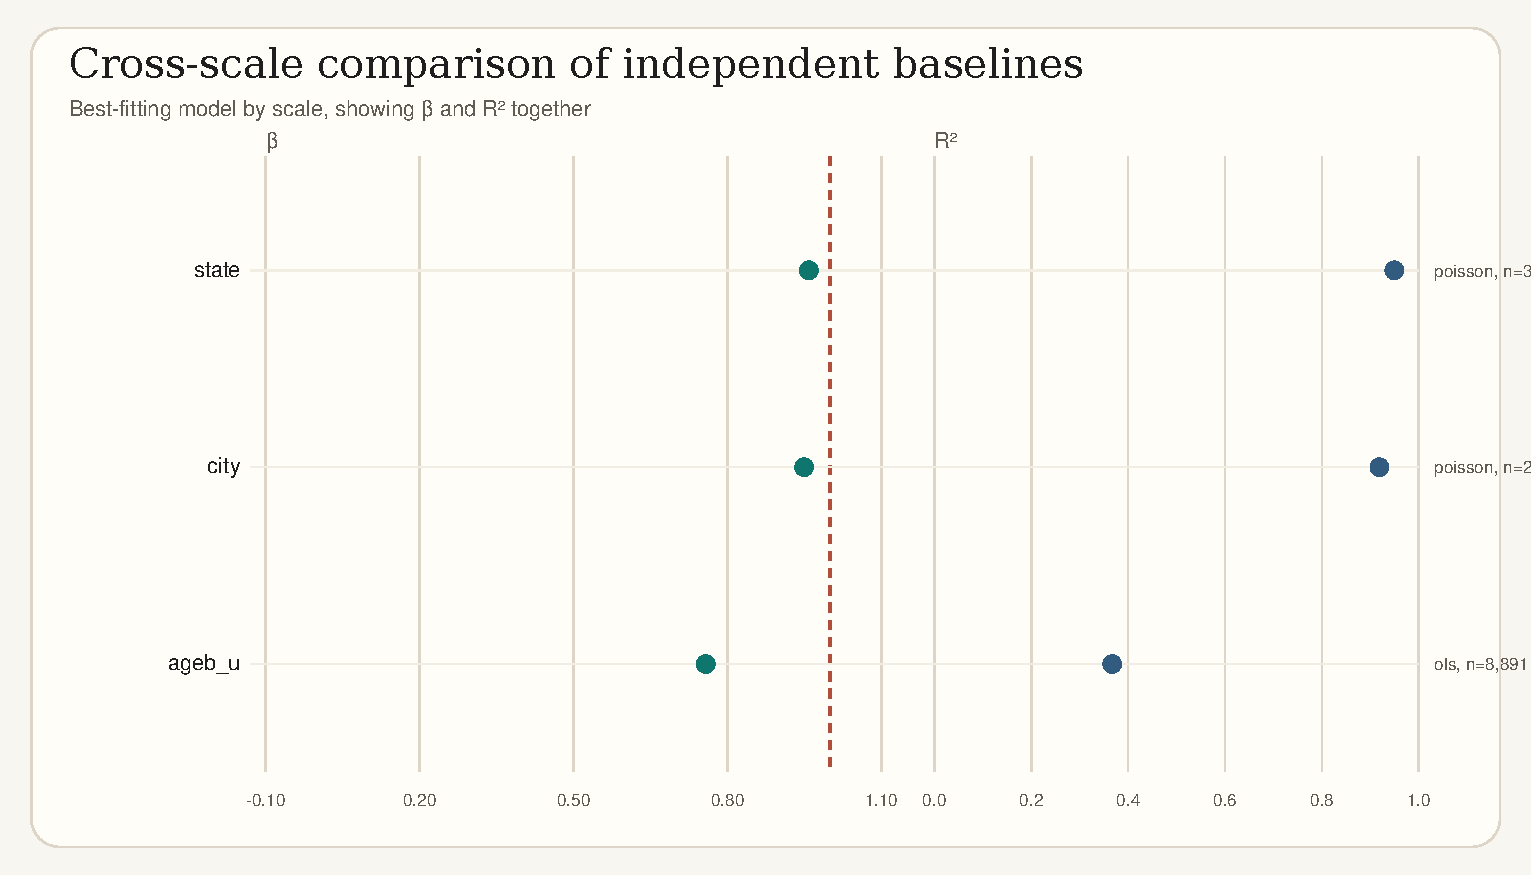
\includegraphics[width=\textwidth]{figures/figure1_support_dependence.pdf}
  \caption{\textbf{Support dependence of establishment scaling.} Comparison of the independent best-fit baselines across state, city and urban AGEB support. The figure summarizes the cross-support decline in fit and the shift from near-linear coarse-scale relations to weaker intra-urban scaling.}
\end{figure}

\subsection*{City-level outcome families}
At the city scale, the aggregate establishment law is strong and close to linear. Total establishments scale with city population with $\beta = 0.9496$ and $R^2 = 0.8460$, confirming that population provides a strong baseline predictor of establishment counts across the Mexican urban system. At the same time, the retained SAMI spread remains substantial, with a 90\% range of 2.0973, showing that strong scaling does not eliminate meaningful differences among cities once size is controlled for.

This aggregate law decomposes unevenly across outcome families. Size-based definitions remain the most coherent. All seven \texttt{per\_ocu} bands and all four derived size classes are retained as interpretable city-scale outcomes. At the family level, the median $\beta$ is 0.9694 for \texttt{per\_ocu} and 0.9749 for \texttt{size\_class}, with median $R^2$ values of 0.7570 and 0.7765, respectively. Micro establishments define the cleanest component of the city law: \texttt{per\_ocu 0 a 5 personas} yields $\beta = 0.9443$ and $R^2 = 0.8397$, while the derived \texttt{micro} size class yields $\beta = 0.9458$ and $R^2 = 0.8426$. Larger classes remain usable, but their fit weakens and their residual spread widens.

Sectoral decomposition is interpretable at SCIAN 2-digit, but not uniformly. Of the 23 sectors present in the city data, 20 are retained as strong or usable, whereas agriculture, mining and management of companies are excluded from substantive interpretation because of weak fit and/or insufficient support. The strongest sectoral law is retail: \texttt{46 Retail trade} has $\beta = 1.0017$ and $R^2 = 0.8732$, and it is also the largest category by national share (40.65\% of all establishments). Several service sectors are also strong, including \texttt{81 Other services except government} ($\beta = 1.0454$, $R^2 = 0.8401$) and \texttt{72 Accommodation and food services} ($\beta = 1.0814$, $R^2 = 0.8246$). By contrast, \texttt{61 Educational services} is clearly sublinear ($\beta = 0.7833$, $R^2 = 0.8165$), while \texttt{54 Professional, scientific and technical services} is more superlinear ($\beta = 1.1739$) but less tightly fitted ($R^2 = 0.7507$).

The sectors with the widest retained city separation are not the best-fitting ones. The broadest 90\% SAMI ranges occur in \texttt{31 Manufacturing I} (3.8210), \texttt{32 Manufacturing II} (3.1808) and \texttt{23 Construction} (3.0031). These categories still retain interpretable scaling laws, but their wider deviation ranges indicate that population alone is less sufficient to organize them than it is for retail or broad service sectors.

\begin{figure}[t]
  \centering
  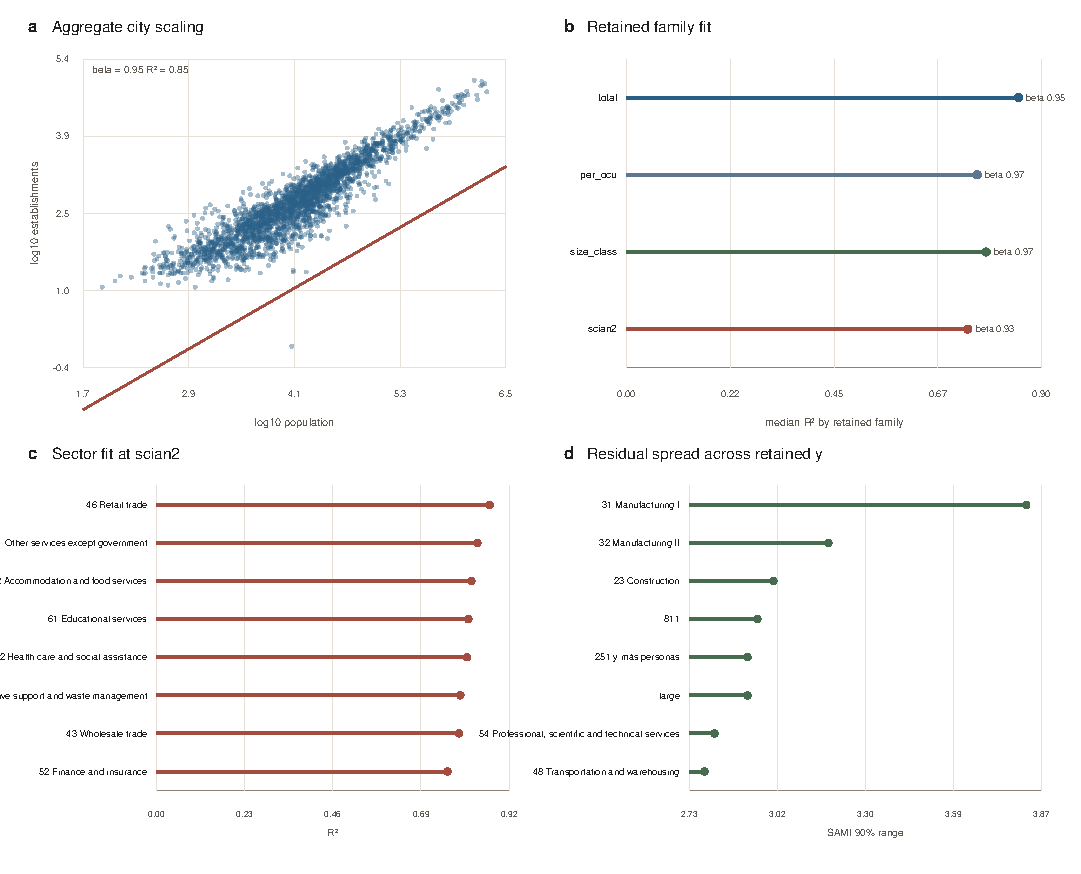
\includegraphics[width=\textwidth]{figures/figure2_city_overview.pdf}
  \caption{\textbf{City scaling and retained outcome families.} The city-scale overview combines the aggregate scaling relation, retained family-level fit quality, sectoral heterogeneity at SCIAN 2-digit and residual spread across retained outcome variables. Together these panels show that the city system preserves a strong aggregate law, but that decomposition by family and sector is heterogeneous.}
\end{figure}

\subsection*{Recurrent city deviations across retained laws}
Once the analysis is restricted to retained city outcomes, recurrent upper-tail and lower-tail deviation profiles become visible. Cuauht\'emoc and Oaxaca de Ju\'arez appear in the upper decile of 41 out of 44 retained city laws, followed by San Pedro Mixtepec (38), Apizaco (34) and Guadalajara (34). At the lower tail, Mezquital appears in the bottom decile of 42 retained laws, followed by Aquism\'on and Tenejapa (37 each), and Chamula and San Jos\'e del Rinc\'on (36 each). These are not isolated category-specific residuals. They identify cities that recur systematically above or below the expected level for size across many retained laws.

This point is central to the interpretation of SAMI. Size-adjusted deviations are not merely leftover noise after fitting the baseline. Strong scaling laws define the expected level for size, while recurrent deviations reveal persistent urban structure around that expectation. The residual hierarchy is therefore substantive: it indicates that some cities repeatedly concentrate more establishments than expected for their size across many retained categories, whereas others repeatedly fall below expectation.

\begin{figure}[t]
  \centering
  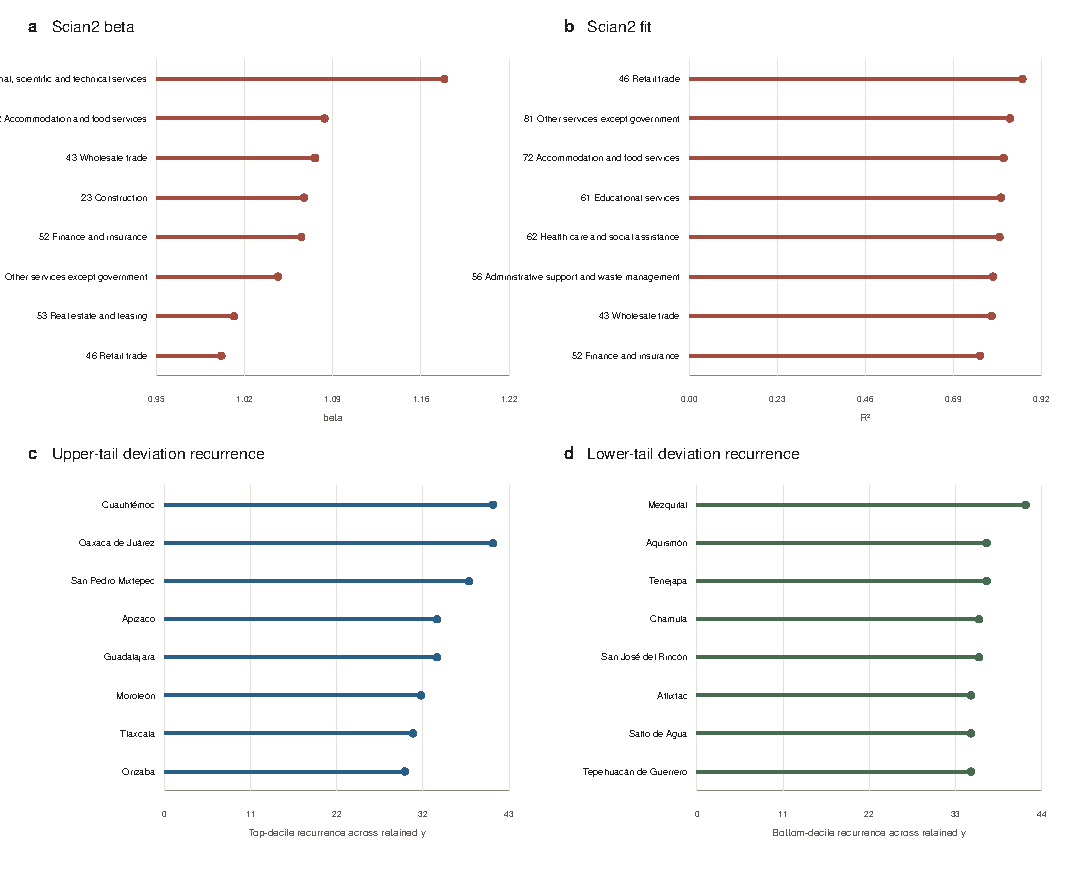
\includegraphics[width=\textwidth]{figures/figure3_city_deviation_profiles.pdf}
  \caption{\textbf{Recurrent city deviations across retained laws.} The figure summarizes sectoral heterogeneity in scaling regime and fit, together with the recurrence of upper-tail and lower-tail size-adjusted deviations across retained city outcomes. These panels show that persistent deviation profiles emerge only after restricting the analysis to interpretable city laws.}
\end{figure}

\section*{Discussion}
The results establish three linked points. First, the Mexican urban system exhibits a strong aggregate city law for establishments, and this city baseline remains the correct theory-native reference point. Second, the apparent strength of the law is support-dependent: coarse aggregation to states tightens the relation, while finer intra-urban support weakens it sharply. Third, decomposition of the city law shows that size-based families are broadly scalable, whereas sectoral heterogeneity becomes interpretable mainly at broad classification levels. Within this retained layer, size-adjusted deviations reveal structured urban differences rather than uninformative residual noise.

These findings suggest a broader research programme. Urban scaling should not be treated as a single exponent attached to a fixed geography. Instead, it should be studied as a support-dependent empirical structure whose fit, meaning and residual hierarchy change across aggregation levels, local geometries and outcome families. In that sense, the city law is not the end of the analysis; it is the baseline from which both aggregation experiments and intra-urban extension experiments become interpretable.

\section*{Methods}
\subsection*{Workflow}
All analyses were executed with the independent \texttt{urban-sami} workflow. The workflow ingests raw DENUE bulk establishment files and official INEGI denominators, constructs support-specific unit tables, fits scaling models of the form $\log(Y) = \alpha + \beta \log(N) + \epsilon$, and computes the canonical SAMI quantity as the raw log deviation $\log(Y/Y_{\mathrm{expected}})$. A secondary standardized diagnostic is also retained, but is not the primary score used in the paper.

\subsection*{Data}
The establishment data come from national DENUE bulk files (\citealp{denue}). Population denominators and administrative codes come from official INEGI sources, including the municipality catalog service and urban AGEB geometry services (\citealp{inegi_catalogo}). The current independent support baselines comprise 32 states, 2,469 municipalities or territorial demarcations with positive population and establishment counts, and 8,891 urban AGEB units in the top-20 municipality sample.

\subsection*{Outcome screening}
At the city scale, a broad catalog of establishment outcomes was constructed from total counts, establishment-size definitions and SCIAN categories. Fitability screening was then applied to retain only outcomes that were interpretable under the scaling framework. This step excluded outcomes with poor support, extreme sparsity or weak fit. Interpretation of residual structure was restricted to the retained subset.

\subsection*{Interpretation}
The city scale was treated as the primary theory run. State was treated as a coarse aggregation experiment over cities, and AGEB as an intra-urban extension experiment. Therefore, deviations were only compared within the same outcome definition and support, and not treated as directly commensurate across different geometries.

\section*{Data and code availability}
All workflow code, report artifacts and manuscript materials used in this draft are available in the local \texttt{urban-sami} repository snapshot used for this manuscript build.

\bibliographystyle{unsrtnat}
\bibliography{references}

\end{document}
